\subsection{Julia}

%\begin{figure}[h]
%    
\includegraphics[width=\linewidth]{img/Julia_Programming_Language_Logo.svg.png}
%    \caption{Logo del linguaggio di programmazione Julia}
%    \label{fig:Julia_logo}
%\end{figure}

Julia è un linguaggio di programmazione ad alto livello, 
multi-paradigma e open-source ideato per compiere analisi 
numerica ed effettuare operazioni di computer science in 
maniera rapida e stabile. Julia è nato ufficialmente come 
linguaggio di programmazione nell’anno 2012 con lo scopo di 
fornire uno strumento potente, robusto e veloce tanto se non 
più dei linguaggi considerati in questo ambito lo stato 
dell’arte, ovvero C e Fortran;  ma anche facile da approcciare, 
al contrario dei linguaggi sopra citati. Julia è un linguaggio 
di programmazione scritto in C++ e Scheme, ma gran parte della 
sua composizione è scritta in Julia stesso 
\cite{wiki:Julia_(programming_language)}.

le caratteristiche principali di questo linguaggio sono 
principalmente:
\begin{itemize}
    \item Alte performance: lo scopo per cui Julia è nato è 
    stato quello di offrire un linguaggio estremamente 
    performante con la capacità di poter compilare programmi 
    in codice nativo per molteplici piattaforme grazie 
    all’utilizzo di LLVM

    % \begin{figure}[h]
    %     \begin{center}
    %         
\includegraphics[width=\linewidth]{img/julia_llvm.jpg}
    %         \caption{Esempio struttura Julia e LLVM}
    %         \label{fig:Julia_LLVM}
    %     \end{center}
    % \end{figure}

    \item Dinamico: la scelta di rendere Julia un linguaggio 
    dinamicamente tipizzato lo rende di facile utilizzo in 
    quanto rende molto più semplice il suo approccio anche a 
    chi non ha una base solida di programmazione, in quanto 
    ritorna la stessa sensazione di immediatezza di un 
    linguaggio di scripting. Inoltre questo permette un alto 
    supporto per l’uso interattivo

    % \begin{figure}[h]
    %     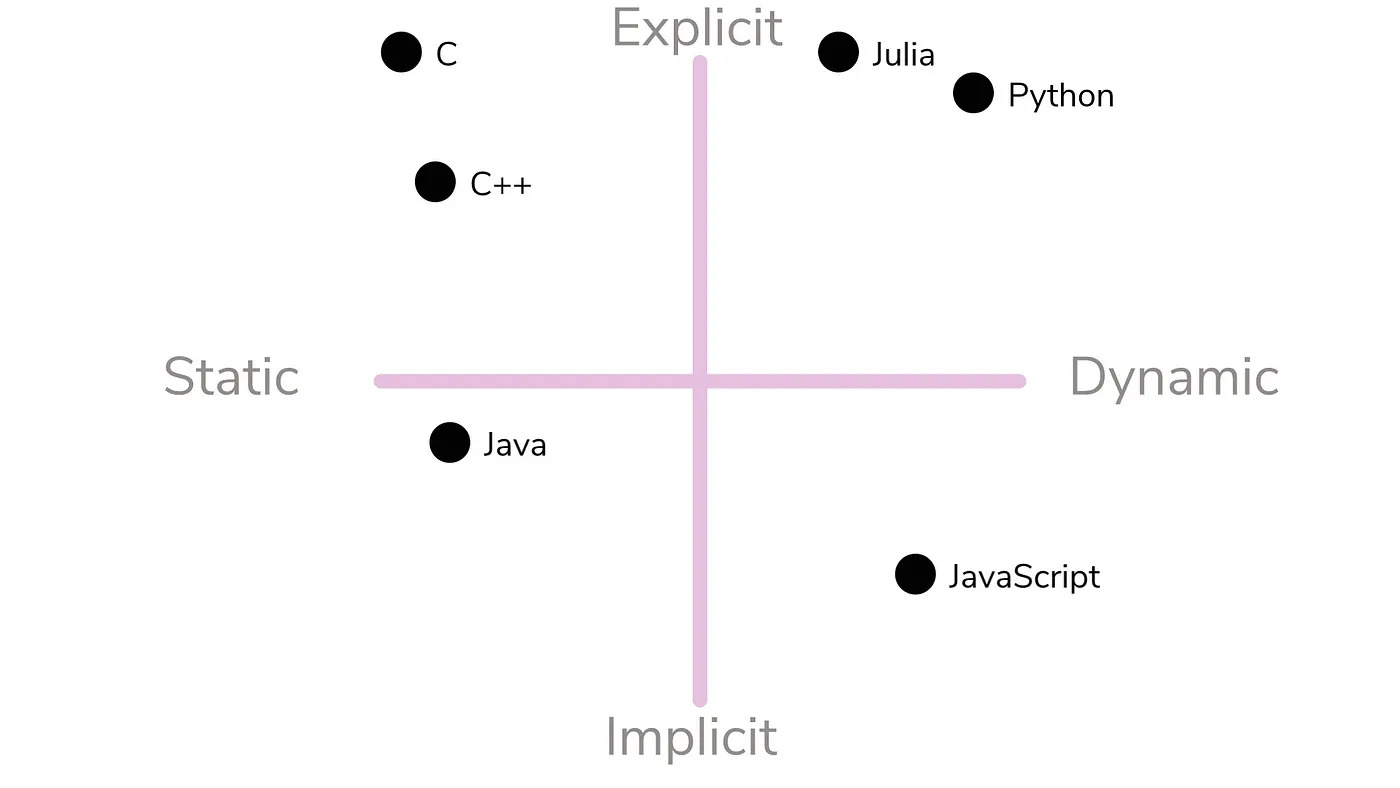
\includegraphics[width=\linewidth]{img/typing_example.jpg}
    %     \caption{Esempio differenze di typing in alcuni linguaggi di programamzione}
    %     \label{fig:Different_typing}
    % \end{figure}

    \item Ambiente riproducibile: lo scopo del linguaggio è 
    quello di poter permettere all’utente di ricreare le 
    stesse condizioni ogni volta su ogni macchina su cui un 
    programma viene eseguito. Questo può essere ottenuto 
    tramite l’utilizzo di file binari pre compilati
    \item Componibile: Julia utilizza l’approccio multiple 
    dispatch come paradigma, permettendo una grande 
    flessibilità nell’esprimere una elevata quantità di 
    pattern di programmazione, dall’object-oriented al 
    funzionale
    \item General Purpouse: lo scopo del linguaggio è quello 
    di creare un ecosistema in grado di poter soddisfare 
    qualsiasi esigenza di un utente, permettendo la creazione 
    di applicativi e microservizi senza dover ricorrere ad 
    integrazioni con codice non nativo Julia
    \item Open source: Julia abbraccia la filosofia open source, 
    e il codice sorgente dell’intero linguaggio, così come di 
    tutte le librerie è disponibile sulla piattaforma GitHub 
    sotto la licenza MIT. Questo permette una crescita 
    eterogenea grazie al contributo di più di 1000 utenti 
    che si impegnano a migliorare il linguaggio
\end{itemize}

\subsubsection{Agents.jl}

%\begin{minipage}{\linewidth}
%    \centering
%    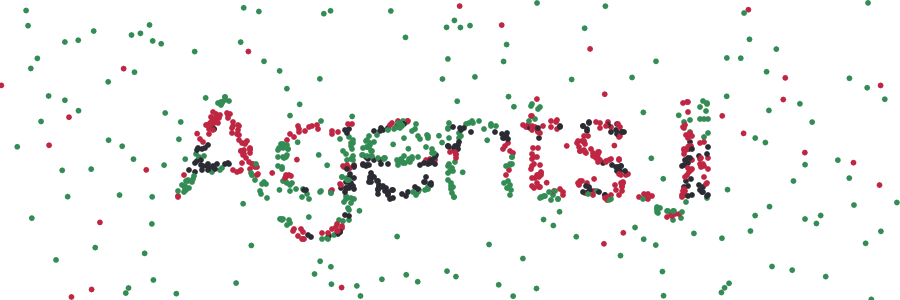
\includegraphics[width=\textwidth]{img/Agents_5poOwRo.png}
%    \captionof{figure}{Logo framework Agents.jl}
%    \label{fig:Agents.jl_logo}
%\end{minipage}

Seguendo la filosofia propria del linguaggio di programmazione 
in cui è sviluppata, la libreria Agents.jl \cite{Agents.jl} 
viene sviluppata con l’obiettivo di essere facile da imparare e 
usare ed estendibile, con forte attenzione sulla creazione ed 
evoluzione di modelli veloci e soprattutto scalabili. 
Molteplici esempi comparativi sono stati effettuati mostrando 
come il framework sviluppato permetta di avere un notevole 
guadagno prestazionale rispetto ai maggiori competitor 
attualmente presenti sul mercato (Mesa, Netlogo, MASON) 
\cite{ABAR201713}.

\begin{minipage}{\linewidth}
    \centering
    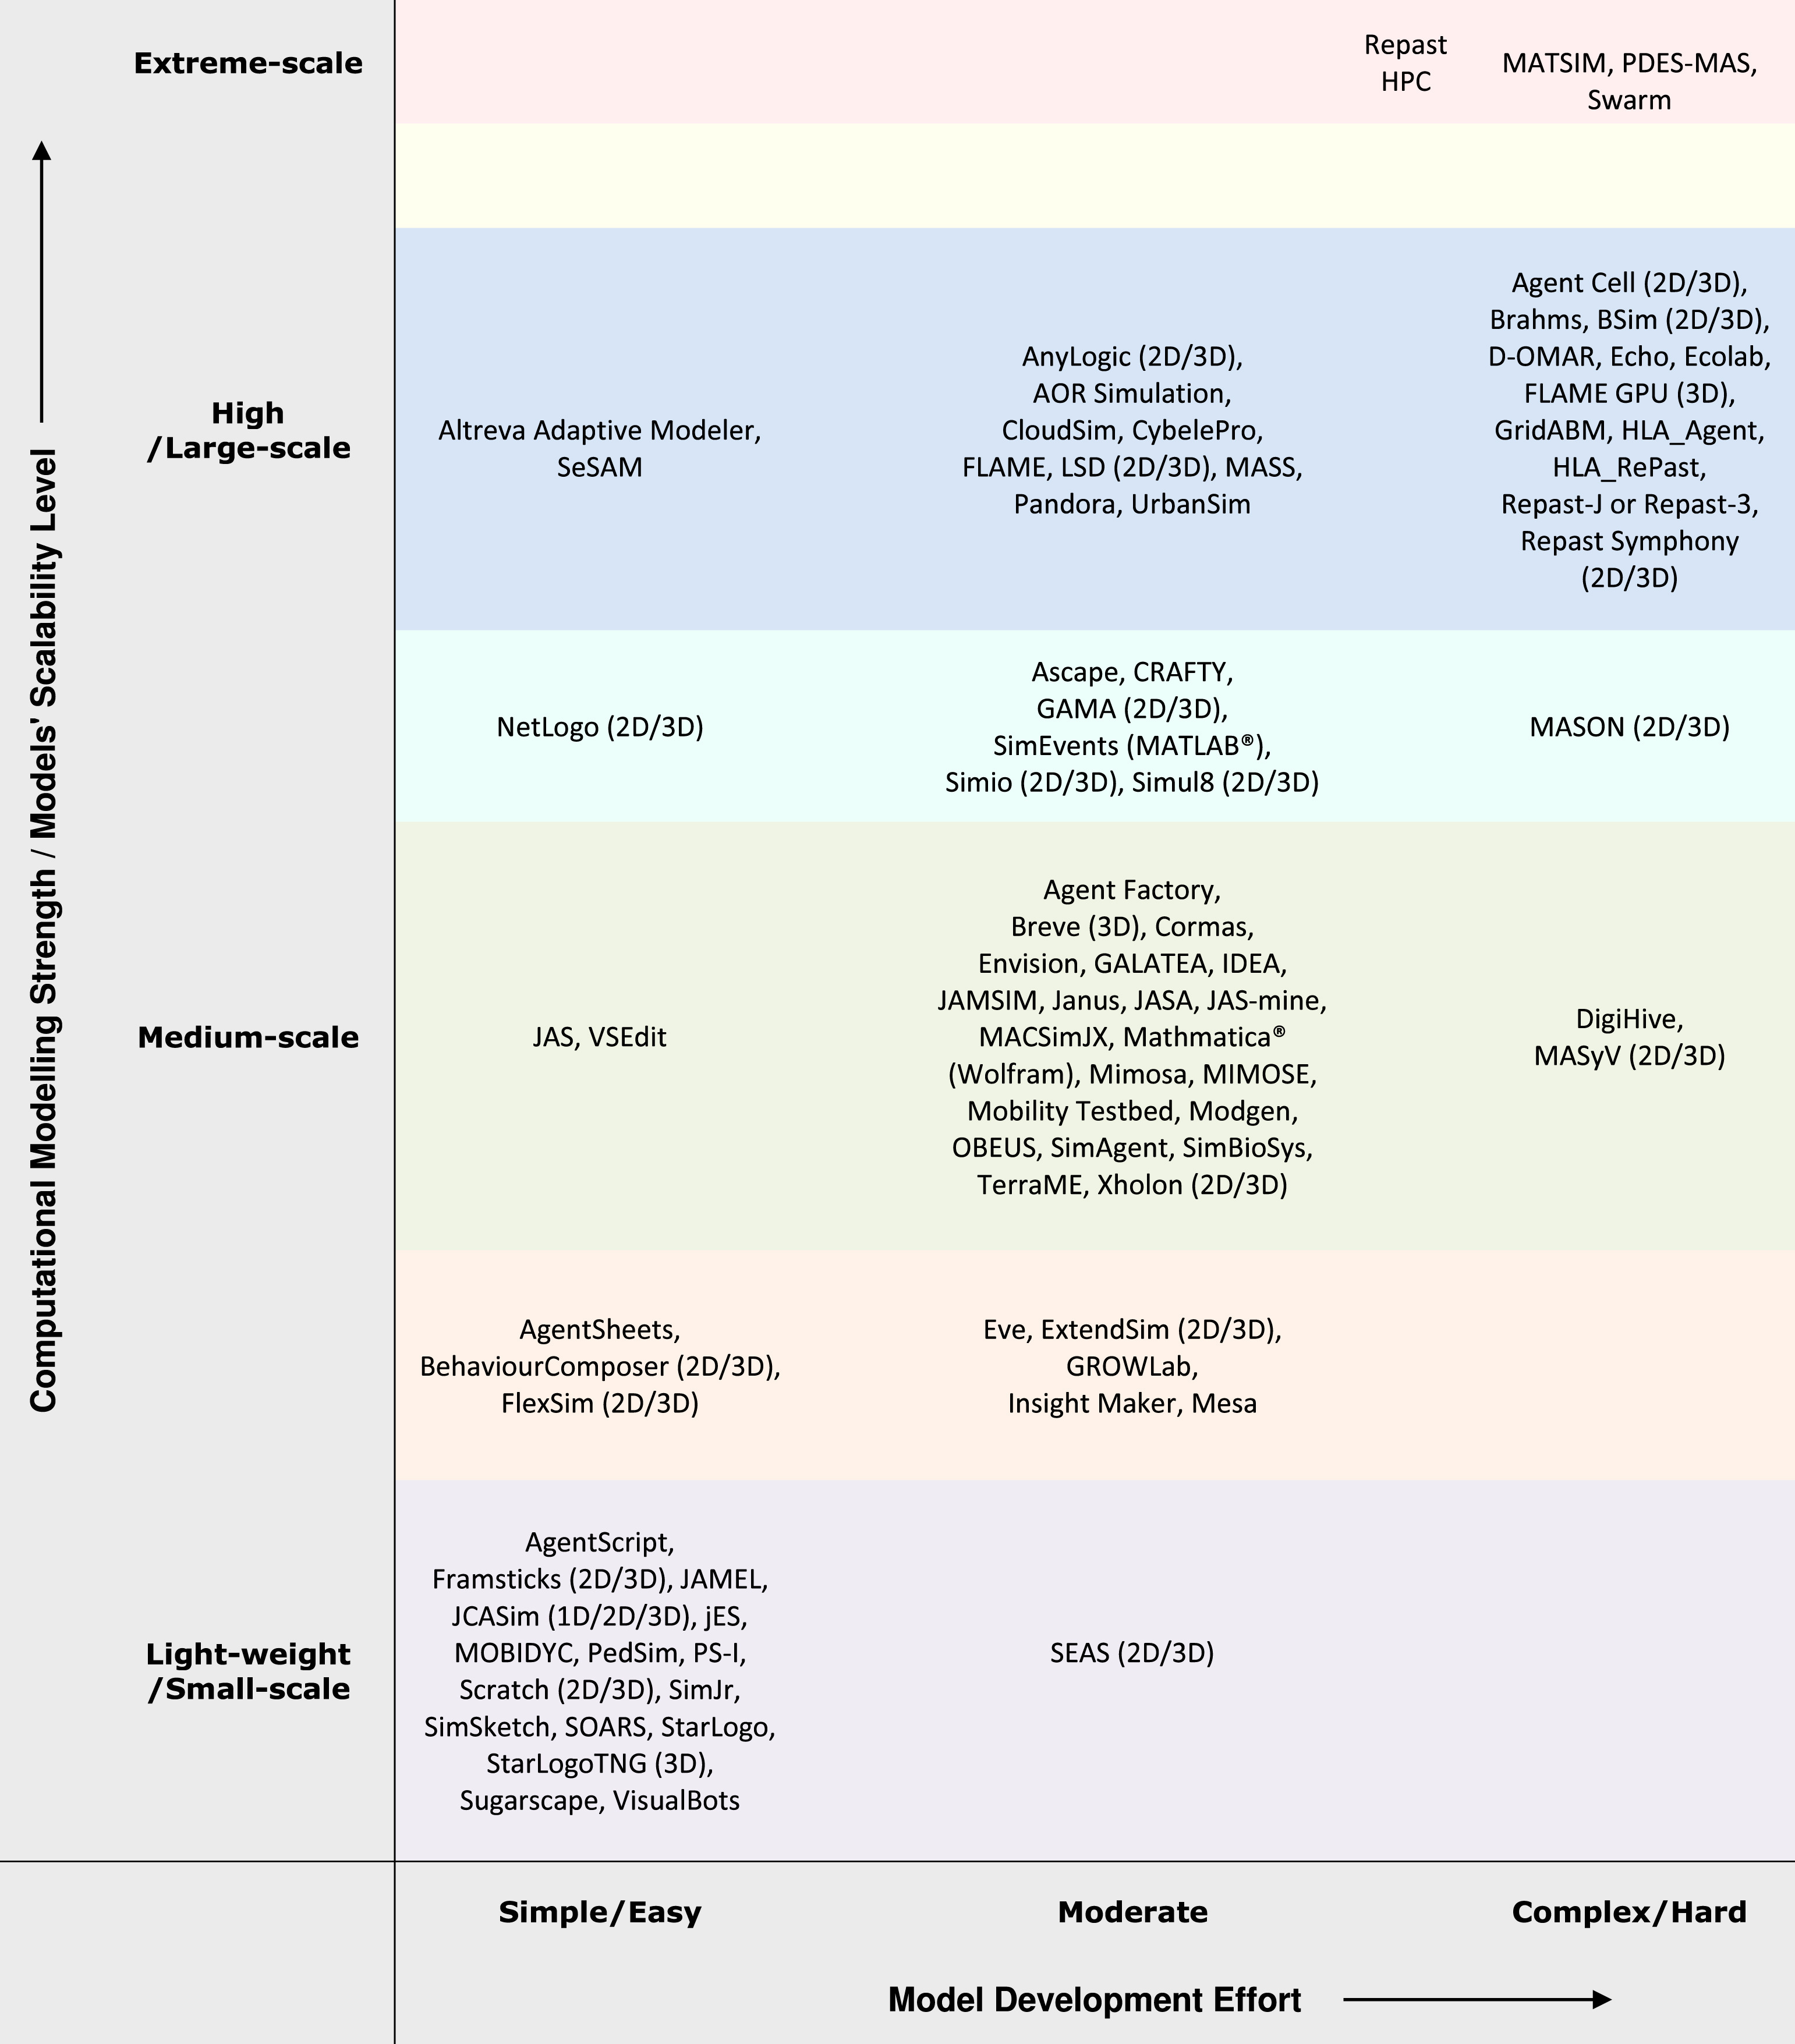
\includegraphics[width=\textwidth]{img/1-s2.0-S1574013716301198-gr1_lrg.jpg}
    \captionof{figure}{Tabella comparativa}
    \label{fig:Comparative_table}
\end{minipage}

La facilità di interazione con questa libreria non è da 
confondersi con una mancanza di opzioni durante lo sviluppo, 
in quanto nativamente Agents.jl permette l’integrazione con 
altre librerie che in maniera altrettanto semplice e veloce 
offrono all’utente la possibilità 
di addentrarsi nel mondo del machine learning, in particolar 
modo il mondo del Scientific Machine Learning 
\cite{rackauckas2017differentialequations}, 
branca che soprattutto grazie alla pandemia da Covid-19 ha 
visto un sempre piu' crescente interesse. 

Agents.jl offre molteplici opzione di configurazione, ma 
principalmente quello su cui si basa sono i seguenti principi:

\begin{itemize}
    \item definizione di un tipo di agente, generalmente viene raccomandato di 
    estendere la tipologia \emph{StandardABM} la quale e' la piu' concreta implementazione,
    nonche' l'implementazione di default, di un costruttore generico di un \textbf{AgentBasedModel}.
    \item definizione di una tipologia di spazio, esistono principalmente 2 tipologie 
    di spazio da poter utilizzare come base e si basano sull'utilizzo di uno spazio \emph{discreto}
    oppure \emph{continuo}.
    \begin{itemize}
        \item spazio discreto a grafo: un \emph{GraphSpace} rappresenta uno spazio del modello
        rappresentato da un grafo arbitrario in cui ogni nodo puo' contenere una 
        quantita' di agenti abitraria. Per funzionare correttamente questa tipologia di 
        spazio richiede che gli agenti implementino al loro interno specifici attributi
        per rappresentare la loro posizione all'interno dello spazio. Questa tipologia di spazio
        si appoggia alla libreria \textbf{Graphs.jl} \cite{Graphs2021} per gestire tutte le operazioni relative
        alla struttura dati del grafo.  

        \begin{minipage}{\linewidth}
            \centering
            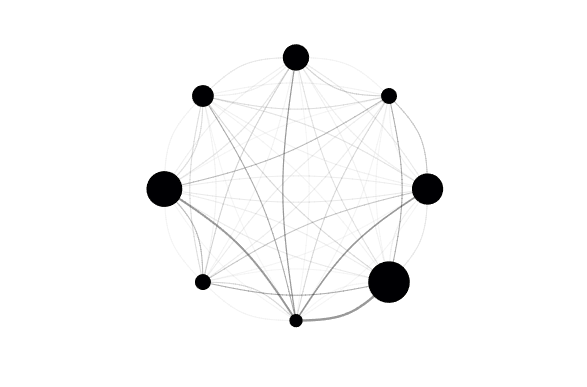
\includegraphics[width=\textwidth]{img/graph.png}
            \captionof{figure}{Rappresentazione di uno spazio a grafo}
            \label{fig:graphspace_representation}
        \end{minipage}
        
        \item spazio discreto a griglia: un \emph{GridSpace} rappresenta uno spazio del modello
        rappresentato da una griglia di dimensione D $\geq$ 1. Questa tipologia di spazio 
        richiede l'utilizzo di una metrica per la definizione della distanza
        tra celle di una griglia. Ci sono attualmente tre tipologie di metriche supportate 
        e sono: \emph{Euclidean}, \emph{Manhattan} e \emph{Chebyshev}.

        \begin{minipage}{\linewidth}
            \centering
            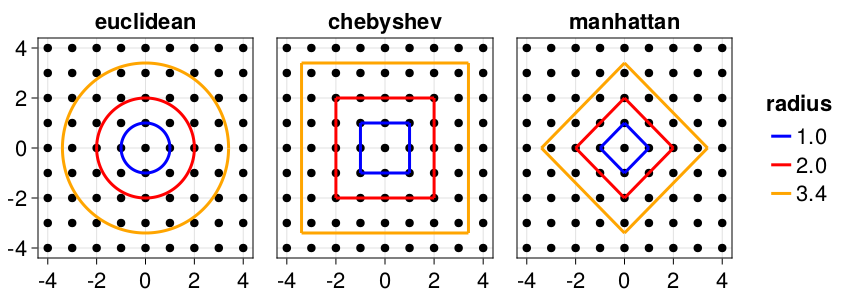
\includegraphics[width=\textwidth]{img/distance.png}
            \captionof{figure}{Metriche di distanza di una griglia}
            \label{fig:gridspace_distances}
        \end{minipage}
        
        \item spazio continuo: un \emph{ContinuousSpace} rappresenta uno spazio di dimensione
        D $\in$ (0, $\infty$). E' fortemente consigliato di attribuire ad un agente all'interno 
        di questo spazio due caratteristiche fondamentali, una posizione e una velocita'. Questa 
        tipologia di spazio permette di rappresentare delle proprieta' spaziali tramite valori 
        finiti oppure tramite \emph{funzioni}, i quali rappresentano una discretizzazione di 
        valori spaziali che potrebbero non essere disponibili in maniera analitica. Utilizzando questa 
        tipologia di spazio la metrica di distanza utilizzata sara' sempre \emph{Euclidian}.
        Per velocizzare il calcolo della posizione degli agenti, viene effettuata una discretizzazione
        implicita dello spazio, ma questa puo' essere forzata a rimanere nello spazio continuo 
        ottenendo un calo di prestazioni.

        \item spazio misto: un \emph{OpenStreetMapSpace} rappresenta una mappa come un'entita' 
        continua che preferisce l'accuratezza alle prestazioni. La mappa viene rappresentata 
        come un grafo connesso. I nodi non rappresentano necessariamente intersezioni. 
    \end{itemize}
\end{itemize} 


\subsubsection{SciML.ai}

\begin{minipage}{\linewidth}
    \centering
    
\includegraphics[width=\textwidth]{img/SciMLGitHubPreview.png}
    \captionof{figure}{Logo SciML.ai}
    \label{fig:SciML.ai}
\end{minipage}

SciML.ai è una collezione di librerie dedite all'analisi numerica e 
e al calcolo scentifico. Questo framework permette di 
avere tutti gli strumenti per poter utilizzare facilmente, 
velocemente e in maniera robusta tecniche di analisi numerica 
molto avanzata, così da poter sviluppare applicazioni complesse 
in maniera semplice e concreta
\cite{rackauckas2017differentialequations} 
\cite{rackauckas2019diffeqflux} 
\cite{rackauckas2020universal}. 

Il principale utilizzo che e' stato fatto di queste librerie si 
concentra principalmente sull'implementazione di metodi di analisi 
numerica, come ad esempio l'utilizzo di di risolutori per sistemi 
di \emph{Equazioni Ordinarie Differenziali} (ODE) che si possono 
trovare nel package \emph{OrdinaryDiffEq.jl} \cite{rackauckas2017differentialequations} 
uniti a metodi di \emph{Machine Learning} (ML) \cite{pal2023lux} \cite{Flux.jl-2018} \cite{innes:2018}
per lo sviluppo di un modello di \emph{Scientific Machine Learning}
\cite{rackauckas2019diffeqflux} \cite{rackauckas2020universal}. 
La principale differenza che esiste tra i modelli classici di ML e quelli 
di SciML e' che i secondi richiedono un numero molto meno elevato di 
dati per la comprensione delle dinamiche che li governano, rendendo questi 
modelli moltio piu' scalabili.

\begin{minipage}{\linewidth}
    \centering
    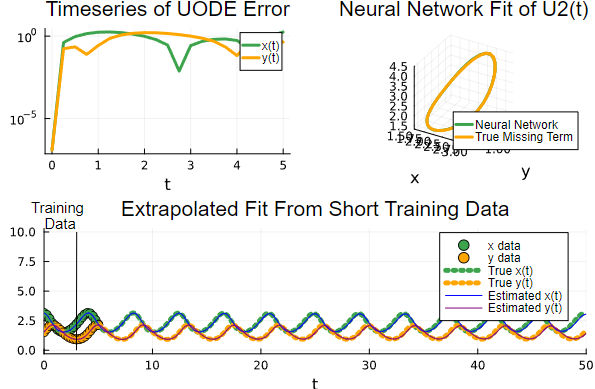
\includegraphics[width=\textwidth]{img/uode_cont.png}
    \captionof{figure}{Esempio di Scientific Machine Learning}
    \label{fig:SciML_example}
\end{minipage}

\subsubsection*{Equazioni Ordinarie Differenziali}
Nell'ambito matematico, una \emph{equazione ordinaria differenziale} (ODE) e' un 
equazione differenziale (DE) dipendente da un singolo valore indipendente, 
generalmente il tempo. All'interno di questa grande famiglia di equazioni, 
il gruppo delle \emph{equazioni lineari differenziali} gioca un ruolo predominante
in quanto la maggior parte dei fenomeni fisici e di matematica applicata possono 
essere descritti dalla soluzione di questo tipo di equazioni. 

Una equazione lineare differenziale e' definita da un \emph{polinomio lineare} 
e la sua derivata e' un equazione dalla forma:

$$\alpha_0(x)y + \alpha_1(x)y' + \alpha_2(x)y'' + ... + \alpha_n(x)y^{(n)} + b(x) = 0$$

dove $\alpha_0(x), ..., \alpha_n(x)$ e $b(x)$ sono funzioni differenziabili arbitrarie che non 
richiedono di essere lineari, e $y', ..., y^{(n)}$ sono le successive derivate della funzione incognita
$y$ della variabile $x$.

L'utilizzo di \emph{equazioni non lineari differenziali} puo' essere 
generalmente approssimato con la controparte lineare cosi' da ottenere una 
soluzione piu' semplice. 

La suite di SciML.ai offre molteplici framework per la risoluzione di sistemi di 
equazioni lineari differenziali prevalentemente all'interno delle librerie 
\emph{DifferentialEquations.jl} \cite{rackauckas2017differentialequations}
\cite{rackauckas2019confederated} \cite{9622796} \cite{gowda2019sparsity},
questi sono separati nelle seguenti categorie:

\begin{itemize}
    \item \emph{Standard Non-Stiff ODEs Solver}
    \item \emph{Standard Stiff ODEs Solver}
    \item \emph{Second Order and Dynamical ODEs Solver}
    \item \emph{IMEX Solvers}
    \item \emph{Semilinear ODEs Solver}
    \item \emph{DAE Solver}
    \item \emph{Misc Solver}
\end{itemize}

\subsubsection*{Equazioni Differenziali Universali}
Un \emph{equazione differenziale differenziale} (UDE) e' una \emph{equazione algebrica
differenziale}\cite{wiki:Differential-algebraic_system_of_equations} 
non triviale, ovvero un sistema di equazioni che contiene delle equazioni differenziali
ed equazioni algebriche oppure e' un sistema equivalente,
con la proprieta' che la sua soluzione puo' approssimare
\emph{qualsiasi} funzione continua su un qualunque intervallo $\in R$ a 
qualsiasi livello di precisione desiderata. \cite{wiki:Universal_differential_equation}

Per essere precisi, una equazione differenziale (possibilmente in forma implicita)
$P( y', y'', y''', ..., y^{(n)})=0$ e' una UDE se, per ogni funzione a valori relative
continua $f$ e per ogni funzione continua positiva $\epsilon$ esiste una 
soluzione liscia\cite{wiki:Smoothness} (una funzione e' considerabile liscia se e' 
differenziabile in ogni suo punto, percio' continua) $y$ di $P( y', y'', y''', ..., y^{(n)})=0$
con $|y(x) - f(x)| < \epsilon(x) \forall x \in R$.

Il concetto di UDE puo' essere analogo all'idea di una \emph{Macchina di Turing Universale}
\cite{wiki:Universal_Turing_machine} con la differenza che le UDE non dettano 
l'evoluzione di un sistema, ma si limitano a imporre determinate regole che 
ogni sistema che si evolve deve sodddisfare. Questo permette di avere un modello robusto 
per l'analisi di dati e la predizione dell'interazione che hanno vari fenomeni tra loro.

\begin{minipage}{\linewidth}
    \centering
    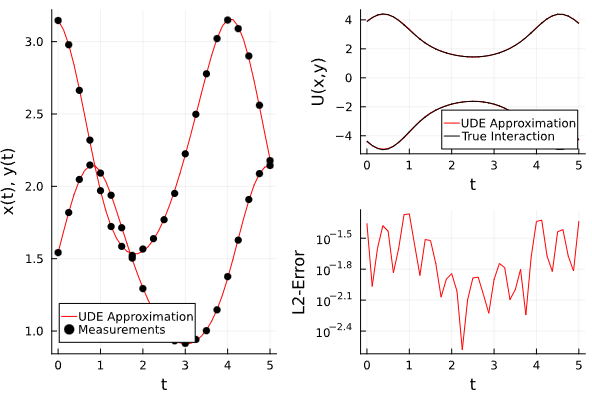
\includegraphics[scale=0.7]{img/ude_approx.png}
    \captionof{figure}{Comportamento UDE nell'approssimazione di fenomeni non lineari}
    \label{fig:UDE_approx}
\end{minipage}

Questo approccio viene spesso unitoa tecniche \emph{Data-Driven} \cite{datadrivendiffeq} per l'identificazione
sparsa di dinamiche non lineari. In particolare uno degli approcci utilizzati 
e' quello tramite l'algoritmo \emph{SINDy} \cite{wiki:Sparse_identification_of_non-linear_dynamics}. 
Questo algoritmo performa una serie di operazioni di regressione come 
ad esempio \emph{LASSO} su una libreria di funzioni candidate non lineari ottenute
da uno snapshot del sistema dinamico che si sta analizzando e delle sue derivate, 
con l'obiettivo di trovare le equazioni che lo governano. Questo procedimento 
si basa sull'assunzione che molti sistemi fisici hanno solamente una manciata di 
termini che ne dettano le dinamiche e l'evoluzione. Questo metodo e' stato largamente
utilizzato nell'identificazione della \emph{dinamica dei fluidi} cosi' come
nelle \emph{reti biologiche} e altri sistemi dinamici complessi.

\subsubsection*{Equazioni Neurali Differenziali}
Recentemente si e' iniziato a ibridare due paradigmi di modellazione come
le ODE e le reti neurali (NN) che hanno sempre avuto ambiti applicativi 
ben distinti, per cercare di ottenere il massimo da entrambe minimizzando 
gli effetti indesiderati. \cite{Kim_2021} \cite{chen2019neural}

L'idea e' quella di inserire una NN come parte sinistra di una ODE, 
e successivamente inserire a sua volta la ODE all'interno di una NN 
piu' grande. Consideriamo il seguente esempio:

$$z(0) = z_0, \frac{dz}{dt}(t) = f_\theta(t,z(t))$$

dove $z_0$ e' un qualsiasi tipo di input, mentre $f_\theta$ e' la nostra rete
neurale, e l'output del modello puo' essere successivamente utilizzato come 
input di $z(T)$ per qualche $T > 0$. Potrebbe sembrare che questo approccio sia
solamente una chimera di due tecniche distinte, quando in verita' non e' cosi. 

Utilizzando i dati ottenuti da una rete neurale, i quali sono stati estrapolati 
dai dati osservati, questi possono essere utilizzati come parametri delle equazioni
differenziali parametriche che costituiscono il modello matematico, unendo la 
flessibilita' di una rete neurale con la robustezza di un modello matematico 
di equazioni differenziali. Questo approccio vede utilizzo in molteplici applicazioni
dal \emph{deep learning} alla tradizionale modellazione matematica. 

Questo tipo di approccio e' \emph{memory efficient}, ha la capacita' di gestire
\emph{dati irregolari} con forti priori sullo spazio del modello, ha un elevata
capacita' di approssimare funzioni lineari e non lineari e si poggia su solide basi 
teoriche che pesca da entrambi i lati.

\begin{minipage}{\linewidth}
    \centering
    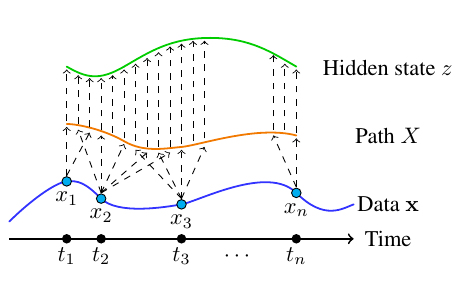
\includegraphics[width=\textwidth]{img/maths-oxford-ml-nde_0.png}
    \captionof{figure}{Esempio di Equazioni Differenziali Neurali}
    \label{fig:NDE_example}
\end{minipage}

\subsubsection{SafeBlues}
Durante la pandemia da Covid-19 il framework SciML.ai è stato 
utilizzato per sviluppare applicazioni le quali grazie 
all’utilizzo di tecniche di scientific machine learning 
riuscivano a prevedere in maniera molto accurata l’andamento 
dell’epidemia, seppur in presenza di una scarsa quantità di dati,
e le stesse presentavano misure di contenimento e prevenzione 
che si sono dimostrate essere efficaci nel loro utilizzo
\cite{10.1371/journal.pdig.0000142} \cite{DANDEKAR2021100220}. 

Un esempio può essere il modello denominato \textbf{SafeBlues} 
\cite{10.1371/journal.pdig.0000142} \cite{DANDEKAR2021100220} 
il quale simulando una rete bluetooth in cui gli individui potevano 
venire infettati da un virus e poi infettare a loro volta gli 
individui circostanti nella rete con una certa probabilità, 
aveva riprodotto fedelmente l’andamento della pandemia da Covid-19. 
In aggiunta questa soluzione, aveva mostrato come 
l’applicazione di policy per il contenimento del virus 
bluetooth erano perfettamente applicabili anche al caso 
reale della pandemia.

\begin{figure}[h]
    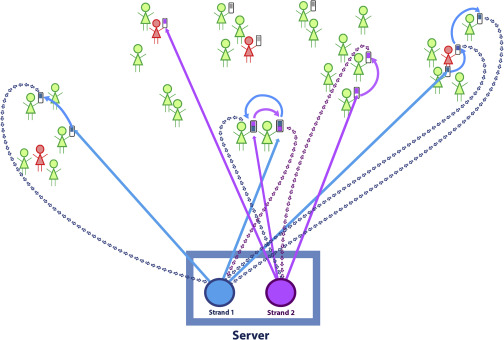
\includegraphics[width=\linewidth]{img/gr2.jpg}
    \caption{Esempio funzionamento SafeBlues}
    \label{fig:SafeBlues_1}
\end{figure}

Questa applicazione e' stata sviluppata e rilasciata per dispositivi
mobili con lo scopo di sperimentare se il sistema svilupatto (\emph{Safe Blues System})
potesse aiutare e migliorare i tradizionali metodi di previsione 
del decorso di una pandemia.